\documentclass[a4paper,12pt]{article}
\usepackage{fullpage}
\usepackage{amsmath,amsthm,amsfonts,amssymb,amscd}
\usepackage{xcolor}
\usepackage{graphicx}
\usepackage{xepersian}


\newcommand{\StudentOne}{4011262134}
\newcommand{\StudentTwo}{4011262098}
\newcommand{\NameOne}{مینا جمشیدی}
\newcommand{\NameTwo}{مبینا محمدی}
\newcommand{\ProjectName}{مستندات پروژه clustering}


\definecolor{CustomBackground}{HTML}{1C1C1C}
\pagecolor{CustomBackground}
\color{white}


\settextfont{Vazir.ttf}[
BoldFont = Vazir-Bold.ttf, 
Path = fonts/]
\setlatintextfont{Vazir.ttf}[
BoldFont = Vazir-Bold.ttf, 
Path = fonts/]


\renewcommand{\baselinestretch}{1.2}
\let\nobreaksection\section
\renewcommand{\section}{\nobreaksection}  % اصلاح شده

\begin{document}
	

	\hrule \medskip
	\begin{minipage}{0.3\textwidth}
		\raggedright
		\small
		\NameOne \\
		\StudentOne \\
		\NameTwo \\
		\StudentTwo
	\end{minipage}
	\begin{minipage}{0.4\textwidth} 
		\centering 
		\large\bfseries
		\ProjectName \\
	\end{minipage}
	\begin{minipage}{0.3\textwidth}
		\raggedleft
		\small
	\end{minipage}
	\medskip\hrule 
	\vspace*{1.5cm}  
	

\section{فاز اول: استخراج ویژگی‌ها}

\subsection*{\textbf{اهداف اصلی}}
هدف از این فاز، پردازش تصاویر طبیعت و استخراج ویژگی‌های کلیدی برای خوشه‌بندی بود. ویژگی‌های استخراج شده باید بتوانند تفاوت بین انواع مختلف تصاویر طبیعی را به خوبی نشان دهند.

\subsection*{\textbf{چالش‌ها و راهکارها}}

\textbf{یکسان‌سازی اندازه تصاویر:}\\
تصاویر ورودی با اندازه‌های مختلف وارد می‌شدند. برای حل این مشکل، همه تصاویر به اندازه استاندارد 128×128 پیکسل تغییر اندازه داده شدند. این اندازه به دلیلی انتخاب شد که هم جزئیات کافی حفظ شود و هم محاسبات بهینه باشد.
\\
\\
\textbf{انتخاب ویژگی‌های معنادار:}\\
ویژگی‌های انتخاب شده باید تفاوت بین کلاس‌ها را به خوبی نشان می‌دادند. برای این منظور از ترکیب چند نوع ویژگی استفاده شد.
\\
\\
\textbf{محاسبه کارآمد ویژگی‌ها:}\\
برای پردازش 3600 تصویر، از توابع بهینه‌شده کتابخانه‌های OpenCV و scikit-image استفاده شد تا محاسبات سریعتر انجام شود.

\subsection*{\textbf{ویژگی‌های استخراج شده}}

\textbf{ویژگی‌های رنگی:}\\
- میانگین کانال‌های R، G، B  
\\
- انحراف معیار کانال‌های رنگی  
\\
این ویژگی‌ها تفاوت رنگ بین مناطق مختلف مثل دریا و جنگل را نشان می‌دهند.
\\
\\
\textbf{ویژگی‌های آماری:}\\
- میانگین سطح خاکستری  
\\
- واریانس سطح خاکستری  
\\
این موارد روشنایی و کنتراست کلی تصویر را اندازه می‌گیرند.
\\
\\
\textbf{ویژگی‌های لبه‌ای:}\\
- تراکم لبه‌ها با فیلتر سوبل  
\\
برای تشخیص مرزهای واضح مثل خط ساحلی مفید است.
\\
\\
\textbf{ویژگی‌های بافتی:}\\
- کنتراست GLCM  
\\
- همگنی GLCM  
\\
این ویژگی‌ها تفاوت بین مناطق یکنواخت و پرجزئیات را نشان می‌دهند.

\subsection*{\textbf{مثال}}

\begin{figure}[h]
	\centering
	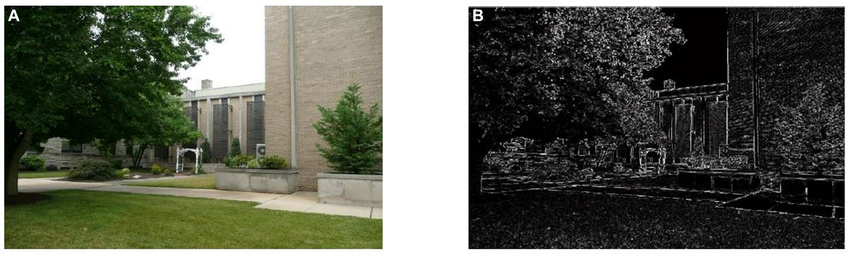
\includegraphics[width=0.8\textwidth]{image1.png}
	\caption{(A) تصویر نمونه, (B) تراکم لبه ها }
	\label{fig:results}
\end{figure}

\subsection*{\textbf{نتایج و خروجی‌ها}}
تمامی ویژگی‌های استخراج شده در فایل features.csv ذخیره شدند.
\\
- 11 ویژگی عددی برای هر تصویر
\\
- برچسب کلاس مربوطه
\\
- امکان استفاده در مراحل بعدی

\subsection*{\textbf{جمع‌بندی}}
ویژگی‌های انتخاب شده:
\\
- تفاوت بین کلاس‌های مختلف طبیعت را نشان دهند
\\
- نسبت به تغییرات جزئی در تصاویر حساس نباشند
\\
- خوب برای مراحل بعدی خوشه‌بندی 
\\
این ویژگی‌ها امکان تفکیک صحیح تصاویر طبیعی را فراهم می‌کنند.
	
	
	\section{فاز دوم: انتخاب ویژگی‌ها}
	
	\subsection{اهداف اصلی}
	\begin{itemize}
		\item انتخاب حداقل 3 ویژگی بهینه از میان ویژگی‌های استخراج شده
		\item محاسبه ماتریس همبستگی بین ویژگی‌ها
		\item تعیین آستانه بهینه برای انتخاب ویژگی‌ها
	\end{itemize}
	
	\subsection{بخش اصلی کد}
\begin{latin}
	\begin{verbatim}
		# Calculate correlation matrix
		def find_correlation():
		# Compute correlations between features
		correlation_matrix = np.zeros((n_features,n_features))
		for i in range(n_features):
		for j in range(i+1, n_features):
		# Correlation calculation formula
		corr = calculate_correlation(i,j)
		correlation_matrix[i][j] = corr
		correlation_matrix[j][i] = corr
		return correlation_matrix
		
		# Select final features
		def select_features(corr_matrix, k=3):
		# Calculate combined score of correlation and variance
		scores = [sum(abs(row))/variance for row,variance in zip(corr_matrix,variances)]
		return np.argsort(scores)[:k]
	\end{verbatim}
\end{latin}
	
	\subsection{نکات کلیدی}
	\begin{itemize}
		\item ماتریس همبستگی به صورت دستی و بدون استفاده از کتابخانه‌های آماده محاسبه می‌شود
		\item معیار انتخاب ویژگی‌ها ترکیبی از میزان همبستگی و واریانس است
		\item تعداد ویژگی‌های انتخابی قابل تنظیم است (پیش‌فرض=3)
	\end{itemize}
	
	\subsection{خروجی‌ها}
	\begin{itemize}
		\item ماتریس همبستگی در فایل \lr{correlation\_matrix.txt}
		\item اندیس ویژگی‌های انتخابی در فایل \lr{selected\_features.txt}
	\end{itemize}
	
	
	\section{فاز سوم: خوشه‌بندی}
	
	\subsection{اهداف اصلی}
	\begin{itemize}
		\item پیاده‌سازی ۴ الگوریتم خوشه‌بندی مختلف
		\item تنظیم پارامترهای هر الگوریتم
		\item مقایسه عملکرد الگوریتم‌ها و انتخاب بهترین روش
		\item تحلیل ویژگی‌های متمایزکننده هر خوشه
	\end{itemize}
	
	\subsection{بخش اصلی کد}
	\begin{latin}
		\begin{verbatim}
			# Initialize clustering algorithms
			algorithms = {
				'KMeans': KMeans(n_clusters=k, random_state=42),
				'Agglomerative': AgglomerativeClustering(n_clusters=k),
				'DBSCAN': DBSCAN(eps=0.3, min_samples=5),
				'MeanShift': MeanShift(bandwidth=0.5)
			}
			
			# Evaluate and compare algorithms
			results = []
			for name, algorithm in algorithms.items():
			labels = algorithm.fit_predict(X_scaled)
			score = silhouette_score(X_scaled, labels)
			results.append({
				'name': name,
				'labels': labels,
				'score': score,
				'n_clusters': len(np.unique(labels))
			})
			
			# Visualize cluster characteristics
			cluster_means = df.groupby('cluster').mean()
			sns.heatmap(cluster_means, annot=True, cmap="YlGnBu")
			plt.savefig("cluster_heatmap.png")
		\end{verbatim}
	\end{latin}
	
	\subsection{نکات کلیدی}
	\begin{itemize}
		\item از معیار \lr{Silhouette Score} برای ارزیابی کیفیت خوشه‌بندی استفاده شده است
		\item داده‌ها قبل از خوشه‌بندی نرمال شده‌اند
		\item نتایج به صورت مصورسازی‌های مختلف ذخیره می‌شوند
		\item برای هر الگوریتم پارامترهای بهینه انتخاب شده‌اند
	\end{itemize}
	
	\subsection{خروجی‌ها}
	\begin{itemize}
		\item فایل \lr{clustered\_results.csv}: داده‌های خوشه‌بندی شده
		\item تصاویر \lr{all\_clustering\_results.png} و \lr{best\_clustering\_result.png}: نتایج خوشه‌بندی
		\item تصویر \lr{cluster\_heatmap.png}: ویژگی‌های متمایزکننده هر خوشه
	\end{itemize}
	
	\section{فاز چهارم: مصورسازی نتایج}
	
	\subsection{اهداف اصلی}
	\begin{itemize}
		\item کاهش ابعاد داده‌ها برای نمایش بهتر
		\item نمایش بصری نتایج خوشه‌بندی
		\item مقایسه روش‌های مختلف کاهش ابعاد
	\end{itemize}
	
	\subsection{بخش اصلی کد}
	\begin{latin}
		\begin{verbatim}
			# PCA 2D Visualization
			pca = PCA(n_components=2)
			X_pca = pca.fit_transform(X)
			plt.scatter(X_pca[:,0], X_pca[:,1], c=labels, cmap='viridis')
			plt.title('PCA 2D Projection')
			plt.savefig('pca_2d.png')
			
			# PCA 3D Visualization
			pca_3d = PCA(n_components=3)
			X_pca_3d = pca_3d.fit_transform(X)
			fig = plt.figure()
			ax = fig.add_subplot(111, projection='3d')
			ax.scatter(X_pca_3d[:,0], X_pca_3d[:,1], X_pca_3d[:,2], c=labels)
			plt.savefig('pca_3d.png')
			
			# t-SNE Visualization
			tsne = TSNE(n_components=2, random_state=42)
			X_tsne = tsne.fit_transform(X)
			plt.scatter(X_tsne[:,0], X_tsne[:,1], c=labels, cmap='coolwarm')
			plt.title('t-SNE Projection')
			plt.savefig('tsne_2d.png')
		\end{verbatim}
	\end{latin}
	
	\subsection{نکات کلیدی}
	\begin{itemize}
		\item از دو روش کاهش ابعاد PCA و t-SNE استفاده شده است
		\item نتایج هم در ۲ بعد و هم در ۳ بعد نمایش داده شده‌اند
		\item رنگ‌های مختلف نشان‌دهنده خوشه‌های مختلف هستند
		\item تصاویر با کیفیت بالا ذخیره می‌شوند
	\end{itemize}
	
	\subsection{خروجی‌ها}
	\begin{itemize}
		\item \lr{pca\_2d.png}: نمایش دو بعدی با PCA
		\item \lr{pca\_3d.png}: نمایش سه بعدی با PCA
		\item \lr{tsne\_2d.png}: نمایش دو بعدی با t-SNE
	\end{itemize}
	
	\subsection{تحلیل نتایج}
	\begin{itemize}
		\item PCA برای نمایش کلی ساختار داده مناسب است
		\item t-SNE برای نمایش روابط غیرخطی و حفظ فاصله‌های محلی بهتر عمل می‌کند
		\item نمایش سه بعدی می‌تواند بینش بهتری از توزیع داده‌ها ارائه دهد
	\end{itemize}
	
	
	\section{فاز پنجم: ارزیابی خوشه‌بندی}
	
	\subsection*{\textbf{اهداف اصلی}}
	در این فاز، عملکرد الگوریتم‌های خوشه‌بندی با معیارهای مختلف ارزیابی شد. هدف اصلی سنجش کیفیت خوشه‌بندی انجام شده و تحلیل نتایج بود.
	\subsection*{\textbf{نتایج اجرای برنامه}}
	خروجی کنسول پس از اجرای کد:
	
	\begin{latin}
		\begin{verbatim}
			Clustering Evaluation Results:
			Average Precision: 0.5878
			Average Recall: 0.6033
			Average F1-Score: 0.5964
			Silhouette Score: 0.1472
			
			Confusion Matrix:
			Predicted 0 1 2 3 4 5
			Actual
			beach 21 18 82 0 291 188
			dense_residential 0 318 124 132 24 2
			desert 509 1 8 1 80 1
			forest 0 56 542 0 2 0
			intersection 0 283 47 67 168 35
			sea_ice 5 47 222 1 229 96
			
			Results saved to evaluation_results.csv
		\end{verbatim}
	\end{latin}
	\subsection*{\textbf{معیارهای ارزیابی}}
	
	\textbf{ Silhouette:}
	\\
	این معیار با مقدار 0.1472 نشان می‌دهد که ساختار خوشه‌بندی تا حدی مناسب است، ولی فضای بهینه‌ای بین خوشه‌ها وجود ندارد. این مقدار نشان می‌دهد که برخی نمونه‌ها نزدیک به مرز خوشه‌ها قرار گرفته‌اند.
	\\
	\textbf{ Precision:}
	\\
	با مقدار متوسط 0.5878 نشان می‌دهد که به طور متوسط حدود 58\% از نمونه‌های هر خوشه متعلق به کلاس غالب هستند. این نشان می‌دهد خوشه‌ها تا حدی خالص هستند.
	\\
	\textbf{Recall:}
	\\
	مقدار 0.6033 نشان می‌دهد که حدود 60\% از نمونه‌های هر کلاس در خوشه مربوطه قرار گرفته‌اند.
	\\
	\textbf{F1-Score:}
	\\
	با مقدار 0.5964 نشان می‌دهد که توازن نسبتاً خوبی بین دقت و فراخوانی وجود دارد.
	
	\subsection*{\textbf{تحلیل ماتریس درهم‌ریختگی}}
	- کلاس desert بهترین عملکرد را با 509 نمونه در خوشه صحیح دارد
	\\
	- کلاس beach و sea ice بیشترین اختلاط را نشان می‌دهند
	\\
	- برخی خوشه‌ها (مانند خوشه 3) نمونه‌های کمی دارند

	
	\subsection*{\textbf{تفاوت معیارها}}
	تفاوت بین مقادیر معیارها به دلایل زیر است:
	\\
	- Silhouette بر اساس فاصله‌های هندسی است
	\\
	- Precision/Recall بر اساس تطابق با برچسب‌های واقعی است
	\\
	- برخی مناطق طبیعی (مثل ساحل و یخ دریا) ویژگی‌های مشابهی دارند
	
	\subsection*{\textbf{جمع‌بندی}}
	نتایج الگوریتم خوشه‌بندی:
	\\
	- برای برخی کلاس‌ها (مانند بیابان) عملکرد خوبی دارد
	\\
	- برای کلاس‌های با ویژگی‌های مشابه نیاز به بهبود دارد
	\\
	- به طور کلی ساختار معقولی ایجاد کرده اما جای پیشرفت وجود دارد
	
	\section{فاز ششم: پیش‌بینی خوشه‌ها}
	
	\subsection{اهداف اصلی}
	\begin{itemize}
		\item پیش‌پردازش و نرمال‌سازی داده‌های تست
		\item پیش‌بینی خوشه‌های داده‌های تست با استفاده از مدل KMeans آموزش‌دیده
		\item مصورسازی نتایج برای ۱۰ نمونه تصادفی
		\item ذخیره نتایج در قالب فایل CSV
	\end{itemize}
	
	\subsection{مراحل اجرا}
	
	\subsubsection{بارگذاری مدل و داده‌ها}
	\begin{latin}
		\begin{verbatim}
			# Load selected features and clustered results
			selected_features = [int(line.strip()) for line in open("selected_features.txt")]
			clustered_df = pd.read_csv("clustered_results.csv")
			
			# Load and preprocess training data for scaler
			train_df = pd.read_csv("features.csv")
			X_train = train_df.iloc[:, selected_features].values
			scaler = StandardScaler().fit(X_train)
		\end{verbatim}
	\end{latin}
	
	\subsubsection{پیش‌بینی خوشه‌ها}
	\begin{latin}
		\begin{verbatim}
			# Process test images and extract features
			features_dict = extract_features(image)
			X_test_selected = X_test[:, selected_features]
			X_test_scaled = scaler.transform(X_test_selected)
			
			# Predict clusters
			test_clusters = model.predict(X_test_scaled)
		\end{verbatim}
	\end{latin}
	
	\subsubsection{ذخیره نتایج}
	\begin{latin}
		\begin{verbatim}
			results_df = pd.DataFrame({
				'image_path': test_image_paths,
				'true_class': test_classes,
				'cluster': test_clusters
			})
			results_df.to_csv("test_predictions.csv", index=False)
		\end{verbatim}
	\end{latin}
	
	\subsection{مصورسازی نتایج}
	\begin{itemize}
		\item برای هر یک از ۱۰ نمونه تصادفی:
		\begin{itemize}
			\item نمایش تصویر تست
			\item نمایش ۵ نمونه از خوشه مربوطه
			\item عنوان‌بندی شامل کلاس واقعی و شماره خوشه
		\end{itemize}
		\item ذخیره خروجی در فایل \lr{test\_samples\_with\_cluster\_members.png}
	\end{itemize}
	
	\subsection{خروجی‌ها}
	\begin{itemize}
		\item \lr{test\_predictions.csv}: شامل مسیر تصاویر، کلاس واقعی و خوشه پیش‌بینی شده
		\item \lr{test\_samples\_with\_cluster\_members.png}: مصورسازی نتایج
	\end{itemize}
	
	\subsection{نکات پیاده‌سازی}
	\begin{itemize}
		\item استفاده از همان اسکیلر آموزش‌دیده در فازهای قبل
		\item حفظ ترتیب ویژگی‌ها مطابق با داده‌های آموزش
		\item نمایش نمونه‌های تصادفی برای بررسی کیفیت خوشه‌بندی
		\item قابلیت کار با انواع مدل‌های خوشه‌بندی
	\end{itemize}
\end{document}